\documentclass[12pt,letterpaper]{article}
\usepackage{amsmath}
\usepackage{amsfonts}
\usepackage{appendix}
\usepackage[figurewithin=section,tablewithin=section]{caption}
\usepackage[usenames,dvipsnames]{color}
\usepackage{graphicx}
\usepackage{tabularx}
\usepackage{longtable}
\usepackage{rotating}
\usepackage{booktabs}
\usepackage[bibencoding=utf8, citestyle=authoryear,bibstyle=authoryear,maxbibnames=99]{biblatex}
\bibliography{/home/jsibert/Projects/MyBibtex.bib,/home/jsibert/MendeleyBibTex/library.bib}

\usepackage[pdftex,bookmarks=false]{hyperref}
\hypersetup{pdfauthor={John Sibert}
            pdfsubject={variable transmission and mortality rate estimates}
            pdftitle={Simple SIR Statistical Model}
            pdfkeywords={Covid-19, SIR Model, random effects, TMB}
            }%

\newcommand\doublespacing{\baselineskip=1.6\normalbaselineskip}
\newcommand\singlespacing{\baselineskip=1.0\normalbaselineskip}
\newcommand\help[1]{\color{Magenta}{\it #1 }\normalcolor}
\newcommand\EG{e.g.\ }
\newcommand\perda{$\rm{da}^{-1}$}
\newcommand\SSm{{\tt simpleSIR4}}
\newcommand\slI{$\sigma_{\ln I}$\ }
\newcommand\slD{$\sigma_{\ln D}$}
\newcommand\slB{$\sigma_{\ln \beta}$}
\newcommand\slM{$\sigma_{\ln \mu}$}

%\renewcommand{\appendixtocname}{Supplementary Material}

\title{Trends in transmission and mortality rates of the Covid-19
pandemic estimated from publicly available data}

\author{
John Sibert\thanks{sibert@hawaii.edu; johnrsibert@gmail.com}\\
Joint Institute of Marine and Atmospheric Research\\
University of Hawai`i at M\={a}noa\\
Honolulu, HI  96822 U.S.A.\\[0.125in]
\date{\today}
}

\pagestyle{headings}
\markright{John Sibert \hfil Covid-19 Transmission \& Mortality \hfil \today}

\begin{document}

\maketitle

\doublespacing

\begin{abstract}
A simple compartment model of Covid-19 infections and deaths is
applied to publicly available data. 
The model estimates trends in transmission and mortality rates using
random effects.
Model estimates of infections and deaths match observations closely. 
Trends in transmission rate vary substantially between geographic
areas. Transmission rates were suppressed below 0.007\perda\ by the
end of May in some areas, but rebounded when social constraints
were relaxed in other areas.
Mortality rates of infected individuals with Covid-19 fell to less than
0.001\perda\ in most areas by the end of July.
These results show that publicly available data, often collected and
compiled with different protocols, can be used to quantitatively
estimate trends in transmission and mortality rate.
\end{abstract}

\section*{Introduction}

The sudden advent of the Covid-19 pandemic provoked many political
jurisdictions to advise people to ``shelter in place'' and to practice
``social distancing''. If this advice has been effective, it should be
possible to detect the effects of the advice by comparing changes in
transmission rates over time and between areas. 
SIR models are often applied to the spread of epidemics and have
been applied to the current Covid-19 pandemic
(e.g. \cite{Chen2020,Roques2020}).
These models divide the affected population into three
compartments: susceptible (S), Infected (I) and Recovered (R).
SIR models are
usually expressed as coupled ordinary differential equations,
\begin{eqnarray}
\label{eqn:SIR}
\frac{dS}{dt} &=& -\beta\frac{IS}{N} - \mu S\\
\frac{dI}{dt} &=& \hphantom{-}\beta\frac{IS}{N} - \mu I -\gamma I\\
\frac{dR}{dt} &=&  -\mu R +\gamma I\\
N &=& S + I + R
\end{eqnarray}
where $N$ is the population size, $\beta$ is the instantaneous
transmission rate ($[t^{-1}]$), $\mu$ is the instantaneous mortality rate
($[t^{-1}]$),
and $\gamma$ is the instantaneous recovery rate ($[t^{-1}]$).  

%https://en.wikipedia.org/wiki/Compartmental_models_in_epidemiology

As the pandemic began to unfold, scientific institutes and governments
at different levels began to make data publicly available on the
World Wide Web.
Data collection protocols vary between institutions and over time, 
and few data sets include data for each of
the compartments in a SIR model. 
The New York Times' ``historical'' 
data set\footnote{\label{ff:nyt}https://github.com/nytimes/covid-19-data/}
is an easily accessible source of data and is updated daily. These data
comprise daily totals of ``cases'' and ``deaths'' for each county
in the United States. I assume that the data included as ``cases'' are
a reasonable approximations of the Infected compartment ($I$) in a SIR
model. There are no credible data of comparable scope on
either the Susceptible or the Recovered compartments.

\section*{Model Structure}
I make some simplifying assumptions in the face of incomplete data: 
(1) The entire population is susceptible so that $S/N = 1$. 
(2) Over the short term, the size of the
Susceptible compartment does not change, 
$\frac{dS}{dt} = 0 = \frac{dN}{dt}$,
eliminating the Susceptible compartment.
(3) People who recover from Covid-19 infections return to the Susceptible
compartment, eliminating the Recovered compartment. 
With these assumptions, and with the addition of a ``deaths''
compartment, the simplified SIR model is
\begin{eqnarray}
\label{eqn:sSIRI}
\frac{dI}{dt} &=&  \beta I - \mu I -\gamma I\\
\label{eqn:sSIRD}
\frac{dD}{dt} &=& \mu I
\end{eqnarray}
Most importantly this model
has state variables that might be matched to available observations.

The available data contain measurement errors of various types.
Definitions and methods of detecting and reporting the numbers of
infected persons and numbers of deaths attributable to Covid-19 have
changed since January of 2020, are continuing to evolve, and can be
expected to change in the future.
Reporting protocols also vary between political jurisdictions (or
``geographies'' in the parlance of the New York Times).
Finally, there is additional variability in biosocial
processes that mediate disease transmission.

I implement the simplified SIR model as a state space-model.
State-space models separate variability in the biosocial
processes in the system (transition model)
from errors in observing features of interest
in the system (observation model).
See \cite{Harvey1990}.

The general form of a {\itshape state-space transition model} is
\begin{equation}
\alpha_t=T(\alpha_{t-1}) + \Theta_t
\end{equation}
where $\alpha_t$ is the state at time $t$ and 
the function $T$ embodies the dynamics mediating the
development of the state at time $t$ from the state at the previous
time with random process error, $\Theta_t$.

The transition model for the simplified SIR model is constructed from
the explicit finite difference
approximations of equations~(\ref{eqn:sSIRI}) and~(\ref{eqn:sSIRD}) 
with associated log-normal
random errors.
\begin{eqnarray}
\label{eqn:sSIRfdI}
I_t &=& I_{t-\Delta t}\big(1+\Delta t(\beta_{t-\Delta t} - \mu_{t-\Delta t}
- \gamma_{t-\Delta t})\big)e^{\eta_t}\\
\label{eqn:sSIRfdD}
D_t &=& \big(D_{t-\Delta t} + \Delta t \mu_{t-\Delta t}I_{t-\Delta
t}\big)e^{\eta_t}
\end{eqnarray}
where $\eta$ is a normal random deviate, $\eta\sim
N(0,\sigma_\eta)$, representing temporal variability in the biosocial
factors that mediate the spread of the pandemic. 
I have no particular justification, beyond the parsimony principle,
for the assumption that the standard deviaton, $\sigma_\eta$, of the processes
for $I$ and $D$, should be the same.

The rate constants in the SIR model differential equations (in this
case $\beta$, $\mu$ and $\gamma$) are often assumed to be invariant.
This biological assumption clearly conflicts with the social
assumptions
that behavioral modification can reduce transmission rates and
that medical advances can reduce both transmission and mortality
rates.
One approach to modeling time-dependent rates of transmission and
mortality, $\beta$ and $\mu$, is to treat them as random effects
(\cite{Skaug2006}). Random effects are appropriate if repeating a time
series of observations would not yield the same outcome as the initial
observations. Random effects are also appropriate when observing
the same process in two different areas. I model the  $\beta$ and
$\mu$ time series as log-normal random walks, and I assume that
\begin{eqnarray}
\log\beta_t &=& \log\beta_{t-\Delta t}+\varepsilon;\quad \varepsilon\sim 
N(0,\sigma_\beta)\\
\log\mu_t &=& \log\mu_{t-\Delta t}+\varrho;\quad \varrho\sim
N(0,\sigma_\mu)
\end{eqnarray}
A similar approach has been used by fisheries scientists to represent
ill-determined parameters in fisheries stock assessment models, such
as time-dependent fishing induced mortality
(\cite{Nielsen2014b,Sibert2017}).
The recovery rate, $\gamma$, in the SIR model is a potential model
parameter, but there are no data with which to constrain it.
Rather, $\gamma_{t-\Delta t}$, in equation~
(\ref{eqn:sSIRfdI}) can be set arbitrarily to 0 or computed algebraically as
\begin{equation}
\label{eqn:gamma}
\gamma_{t-\Delta t} = \beta_{t-\Delta t} - \mu_{t-\Delta t} +
(1-\frac{I_t}{I_{t-\Delta t}})
\end{equation}

The general form of the {\itshape state-space observation model} is
\begin{equation}
x_t = O(\alpha_t) + \Omega_t
\end{equation}
where the function $O$ describes the measurement process with
error $\Omega$ in observing the state $\alpha$.

I applied separate observation error models for cases and
deaths. The observation model for cases is a simple log-normal error
\begin{equation}
\label{eqn:logNlike}
\log\varphi_t = \bigg(\log\frac{1}{\sqrt{2\pi\sigma^2_I}} -\Bigl(\frac{\log
I_t-\log\widehat{I}_t}{\sigma_I}\Bigr)^2\bigg)\\
\end{equation}
where $I$ is the observed number of cases and $\widehat{I}$ is the
number of cases predicted by equation~(\ref{eqn:sSIRfdI}).


Not all those afflicted by Covid-19 have died; there are far fewer
deaths than infections. In addition,
the observed time series for both $I$ and $D$ begins at the first recorded
case, i.e., at time $t=0, I_t \ge 1$. The first recorded death occurs
several days or weeks after the first recorded case.
Therefore the deaths time-series inevitably contains a
substantial number of initial recorded zeros. 
The observation model for deaths is a ``zero-inflated'' log normal
error to accommodate observed zeroes
\begin{equation}
\label{eqn:ZIlogNlike}
  \log \varepsilon_t = \left\{
    \begin{array}{r@{\;:\quad}l}
       D_t > 0 &
(1-p_0)\cdot\bigg(\log\frac{1}{\sqrt{2\pi\sigma^2_D}}
          -\Bigl(\frac{\log D_t-\log\widehat{D}_t}{\sigma_D}\Bigr)^2\bigg)\\
       D_t = 0 & p_0 \cdot\log \frac{1}{\sqrt{2\pi\sigma^2_D}}\\
    \end{array}
  \right.
\end{equation}
where $D$ is the observed number of deaths,
$\widehat{D}$ is the number of deaths predicted by
equation~\ref{eqn:sSIRfdD}, 
and $p_0$ is the proportion of observed deaths equal to zero.

Model parameters are estimated by
maximizing the joint likelihood of the process errors, observation
errors, and random effects.
\begin{equation}
\label{eqn:likelihood}
L(\theta,\alpha,x)=
\prod^m_{t=1}\big[\phi\big(\alpha_t-T(\alpha_{t-1}), \Theta\big)\big]\cdot
\prod^m_{t=0}\big[\phi\big(x_t-O(\alpha_t), \Omega\big)\big]
\end{equation}
where $m$ is the number of days elapsed since the first recorded case,
$x_t$ is the vector of daily observations of cases and deaths,
$\alpha_t$ is the vector of the daily predictions of cases and deaths,
variables and random effects,
and $\theta$ 
is a vector of model parameters and random effects (Table~\ref{tab:allvars1}).
The R package TMB (\cite{TMB0000}) was used to implement the
simplified SIR model and to 
estimate the model parameters.
All R and C++ source files are available on 
github.\footnote{\SSm~at \url{https://github.com/johnrsibert/SIR-Models}}

\begin{table}[!h]
\caption{List of model variables for the simple SIR model, \SSm.
There are two state variables computed from the of estimated
parameters and random effects.
There are two random effects and five estimated variance parameters.
All models variables are represented in the TMB C++ module as their
natural logarithms.
}
\label{tab:allvars1}
\begin{center}
\begin{tabular}{ll}
\hline
Variable & Definition\\
\hline
\hline
       & {\it State variables:}\\
$I$      & Number of infected individuals\\
$D$      & Number of deaths\\
       & {\it Random effects:}\\
$\beta_t$ & Transmission rate; log-normal random walk\\
$\mu_t$   & Mortality rate; log-normal random walk\\
       & {\it Estimated parameters:}\\
$\sigma_I$ & Infectious compartment estimation standard deviation\\
$\sigma_D$ & Deaths compartment estimation standard deviation\\
$\sigma_\eta$ & Standard deviation of transmission and deaths process errors\\
$\sigma_\beta$ & Standard deviation of transmission rate random walk\\
$\sigma_\mu$ & Standard deviation of mortality rate random walk\\
\hline
\end{tabular}
\end{center}
\end{table}

\clearpage
\section*{Results}

\begin{figure}[h!]
\begin{center}
\includegraphics[width=1.00\textwidth]{../Graphics/constrainID/counties_per_capita.pdf}
\end{center}
\caption{\label{fig:percap}
Trends in number of cases per 1000 people in the 30 most populous US
counties.
The vertical gray bar mark the March 19, 2020 California shelter in place order.
See Table~\ref{tab:namekey} for key to county abbreviations.
}
\end{figure}

%All data are derived from the New York times github 
%site\footnote{See note \ref{ff:nyt}.}.
% {\url{https://github.com/nytimes/covid-19-data/}}. 

Six months after the pandemic began spreading in the United States, it
was obvious that some areas were more successful than other
in controlling the spread of the Covid-19 virus.
Trends in the per-capita number of cases in the thirty most populous 
counties in the United States are shown in Figure~\ref{fig:percap}.
The shapes of these trends form a continuum from those that bend
sharply upward, \EG Miami-Dade Co FL (MDFL),  to
those that appear to reach a plateau, \EG Nassau Co NY (NaNY). 


\begin{figure}
{\scriptsize
\begin{center}
\includegraphics[width=0.80\textwidth]{../Graphics/constrainID/NassauNY_prevalence.png}
 
\vspace{0.5truein}

\includegraphics[width=0.80\textwidth]{../Graphics/constrainID/Miami-DadeFL_prevalence.png}
\end{center}
}
\caption{\label{fig:prev}
Prevalence histories for two US counties.
Blue bars indicate daily increases increases in cases and deaths;
dark blue lines indicate 11 day moving averages of
daily increases (labeled ``11da'');
pale blue lines indicate cumulative numbers of cases and deaths
(labeled $\Sigma C$ and $\Sigma D$); 
vertical gray bar marks the March 19, 2020 California shelter in place order.
}
\end{figure}

Prevalence histories for counties representative of plateau
(Nassau Co NY)
and upward bending (Miami-Dade Co FL) trajectories are shown in
Figure~\ref{fig:prev}. The 11-day moving averages of the daily
increases in cases and deaths is an indicator of the
relative success in controlling the outbreak.
The cumulative trends in number of cases is equivalent to 
the per capita trends in Figure~\ref{fig:percap}.
All histories show extreme day to day variability.
Variability is most notable in the deaths
time series, particularly for smaller counties.
The cumulative deaths trajectory for Nassau County, NY, illustrates
changing reporting practices. The New York Times changed the method of
reporting deaths in New York State 
\footnote{For details see
https://github.com/nytimes/covid-19-data/blob/master/NEW-YORK-DEATHS-METHODOLOGY.md}.
The effect of this change can be seen in the sharp {\itshape drop} in
the cumulative number of deaths on August 6.

The \SSm\  model estimates two random effects and five parameters.
In principle, all random effects and parameters are estimated
simultaneously.
Initial experiments with the model showed that some
numerical algorithms used to find the minimum of the log likelihood
function were unable to reach a solution easily. Minima were reached
for some counties, but most attempts terminated prematurely. 
Inspection of the diagnostic plots for the model showed that predicted
values of cases and deaths matched observed values almost exactly
but with unrealistically low estimates of \slI and \slD, 
figures~\ref{fig:estsNaNYu} and~\ref{fig:estsMDFLu} and table~\ref{tab:uncons}.
These initial experiments made it clear also
that attempting to either compute or estimate
the recovery rate parameter, $\gamma$, in the absence of a counts of
recovered patients is futile. The calculated values of $\gamma$ from
equation~{\ref{eqn:gamma}) were invariably close to 
zero ($\sim 10^{-8})$.

All subsequent analysis fixed the observation model variances to
\slI~$ = 0.223$ and \slD~$= 0.0953$, and $\gamma = 0$.
These standard deviations are equivalent to measurement errors of
approximately 25\% in reporting cases and 10\% in reporting deaths.
The algorithm converges to a solution in all cases, and converges
rapidly using gradient methods.

Diagnostic plots for the constrained model are shown in
figures~\ref{fig:estsNaNYc} and~ \ref{fig:estsMDFLc}
for plateau and upward  bending trajectories respectively.
Estimated cases and deaths agree well with observation throughout the
time series and fall cleanly withing the area bounded by the
constraints on the observation model errors.
Distinct trends in transmission rate estimates are evident for
the two prevalence patterns. A small transitory upward ``bump'' in July is
evident for Miami-Dade Co FL.
In contrast, the estimated transmission rate for Nassau Co NY trends
downward monotonically. 
Estimated mortality rates trend generally downward subsequent to an
initial peak for both prevalence patterns.

\begin{figure}[!h]
\begin{center}
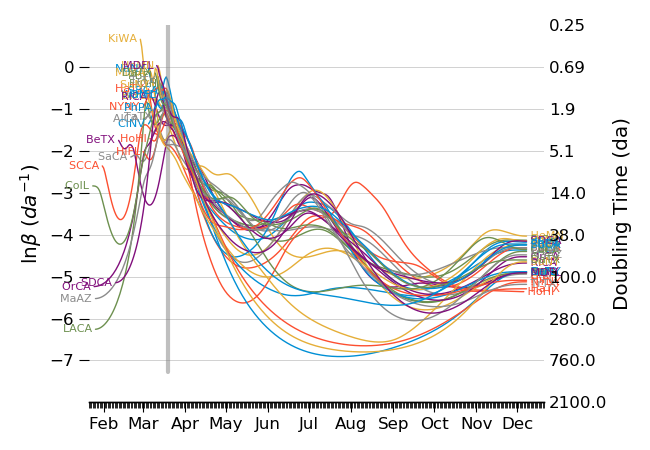
\includegraphics[height=0.50\textheight]{../Graphics/constrainID/logbeta_summary_g.pdf}\\
%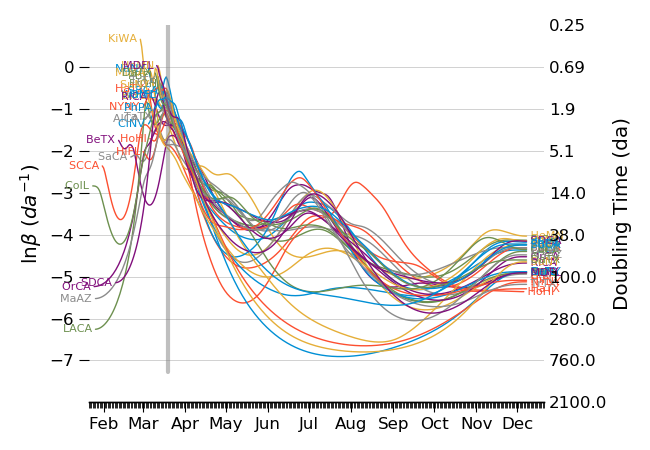
\includegraphics[width=1.00\textwidth]{../Graphics/constrainID/logbeta_summary_g.pdf}\\
\end{center}
\caption{\label{fig:xrates}
Estimated natural logarithms of the transmission rate for thirty two US
counties using the constrained \SSm\ model.
Equivalent doubling times ($t_2 = \frac{\ln 2}{\exp(\ln \beta)}$)
are shown on the right-hand ordinate.
See Table~\ref{tab:namekey} for key to county abbreviations.
}
\end{figure}

Figure~\ref{fig:xrates} compares estimated transmission rate among
counties.
Transmission rates increased rapidly in February and early March for
counties which reported their first cases earlier in the year.
By mid March the instantaneous transmission rate
was greater than 1\perda\ ($\ln \beta \approx 0$) in most counties,
equivalent to a doubling time of less than one day.
Transmission rates fell substantially in April, and doubling times
increased to longer than 20 days in some counties by late May.
Counties with estimated transmission rates less than 0.007\perda\ 
(or $\ln \beta \le 5$) at the end of May
correspond roughly to those counties with plateau prevalence
trajectories.

\begin{figure}[!h]
\begin{center}
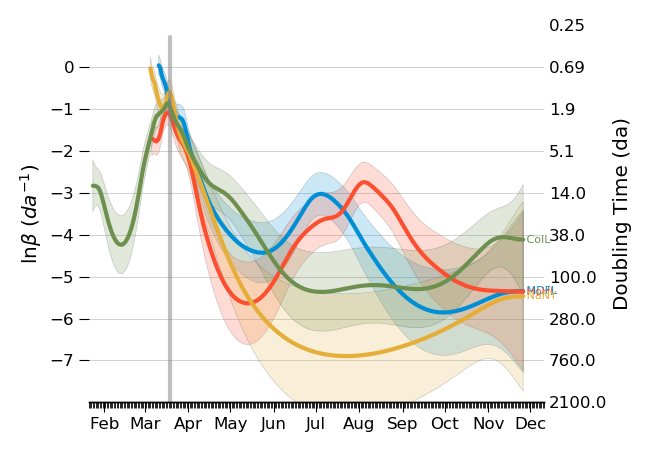
\includegraphics[height=0.50\textheight]{../Graphics/constrainID/logbeta_summary_4.pdf}\\
\end{center}
\caption{\label{fig:xrates2}
Estimated natural logarithms of the transmission rate for four US
counties using the constrained \SSm\ model.
The shaded areas indicate the estimated random effect $\pm 2$
estimated standard errors.
Equivalent doubling times ($t_2 = \frac{\ln 2}{\exp(\ln \beta)}$)
are shown on the right-hand ordinate.
See Table~\ref{tab:namekey} for key to county abbreviations.
}
\end{figure}

Figure~\ref{fig:xrates2} compares transmission rate between counties
with plateau prevalence trajectories (Cook Co, IL and Nassau Co, NY) and
upward  trending trajectories (Honolulu Co, HI and Miami-Dade Co
FL). The Honolulu example indicates that simply suppressing the
transmission rate to a point where the doubling time is greater than
100 days does not ensure sustainable suppression of the spread of the
disease. The regions enclosed
by $\pm 2$ standard errors show that estimated transmission rates
these four counties were similar in April and May, but diverged
significantly in June to become distinct in August.

\begin{figure}[!h]
\begin{center}
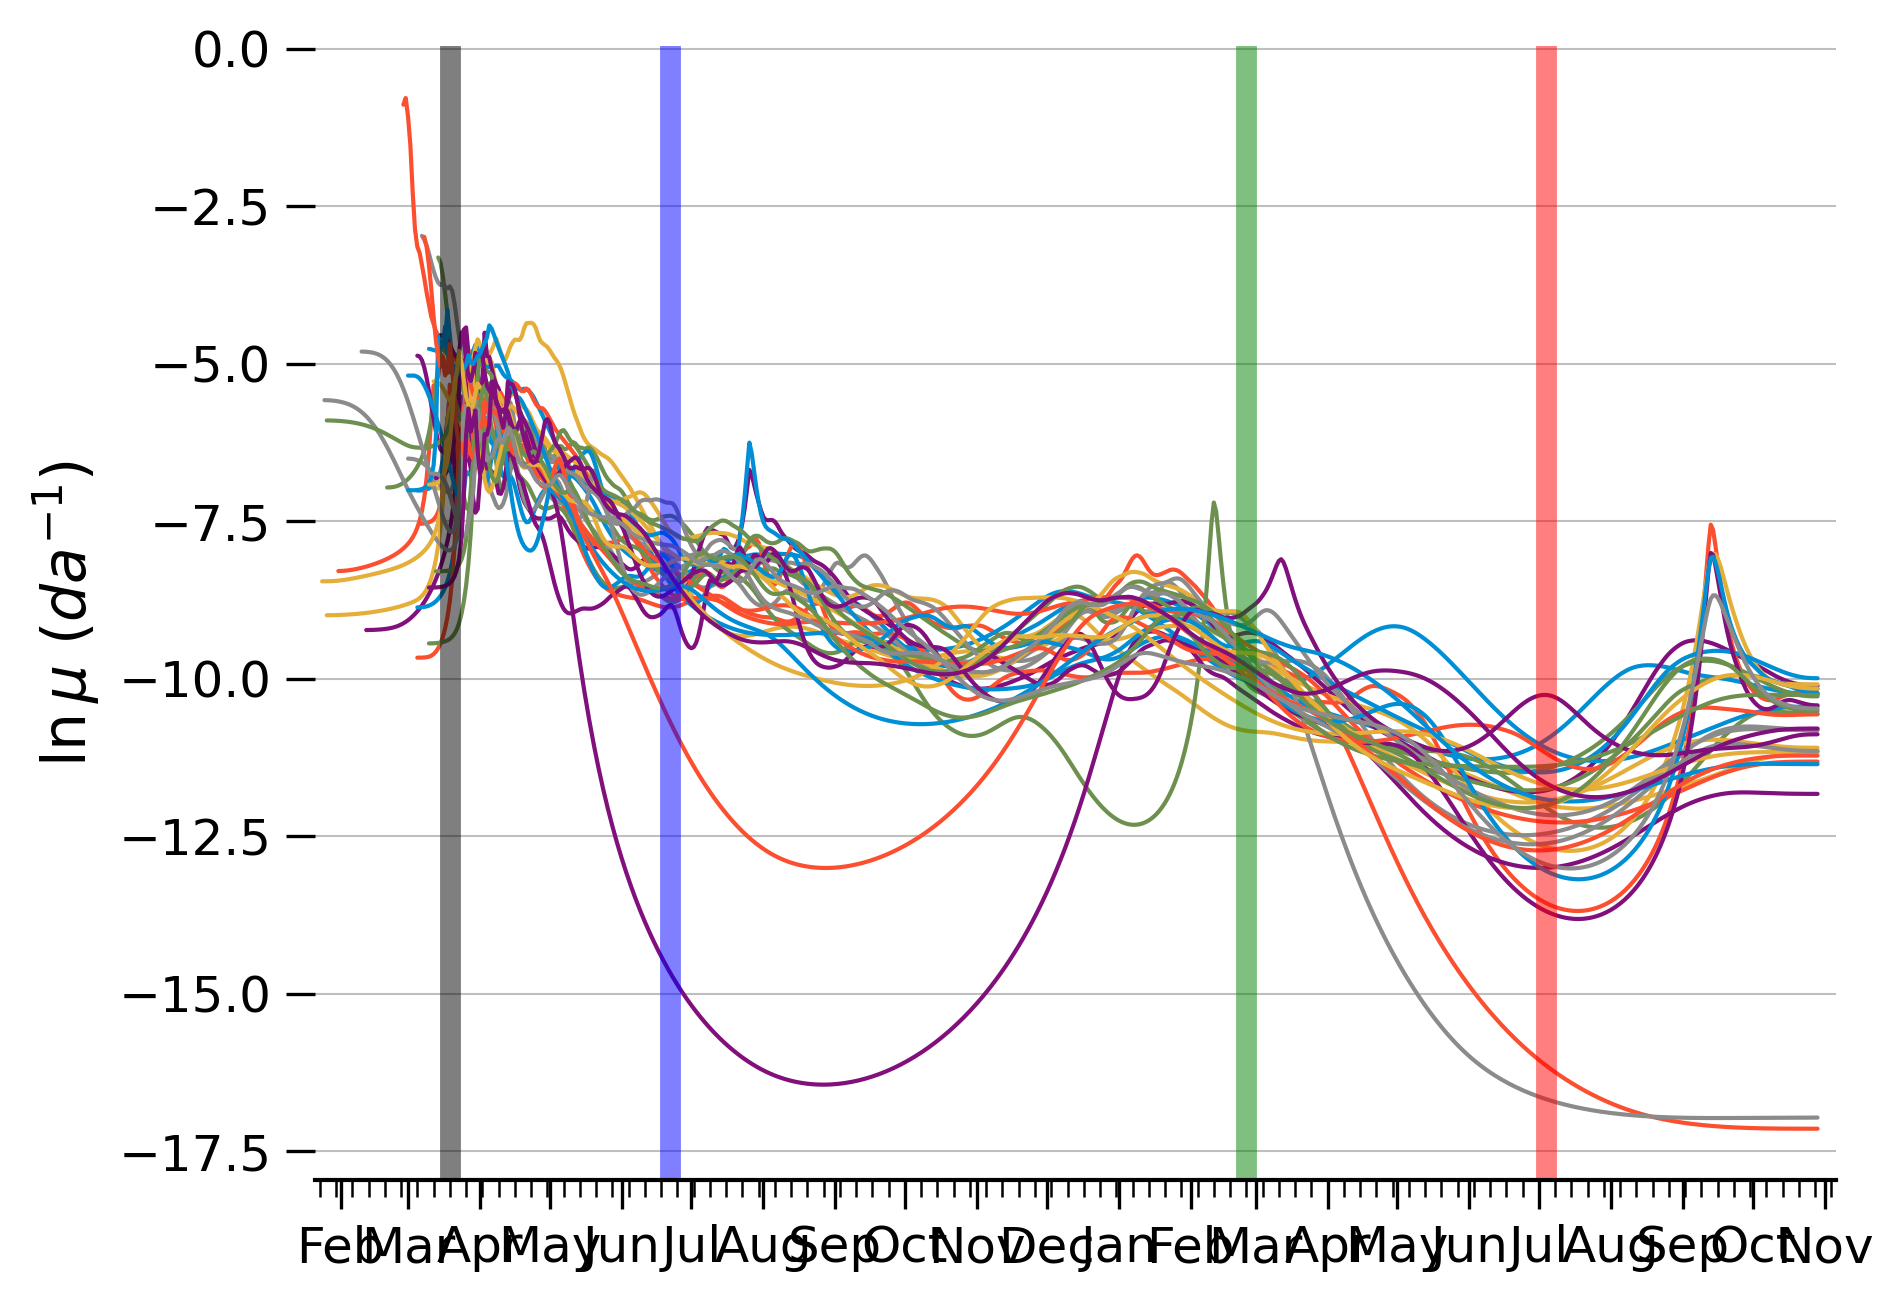
\includegraphics[height=0.50\textheight]{../Graphics/constrainID/logmu_summary_g.pdf}\\
\end{center}
\caption{\label{fig:drates}
Estimated natural logarithms of the mortality rate for thirty two US
counties using the constrained \SSm\ model.
See Table~\ref{tab:namekey} for key to county abbreviations.
}
\end{figure}

Figure~\ref{fig:drates} compares estimated mortality rate among
counties. Initial mortality rates were quite variable during the first
months of the pandemic and but rose quickly to around 
0.01\perda\ ($\ln \mu \approx -4.6$) in April. Subsequently the
estimated mortality rates decreased for all counties and appear to
have leveled off in August to lows near
0.0003\perda\ ($\ln \mu \approx -8$) in August.

%\clearpage
\section*{Discussion}

Nonlinear statistical models with multiple parameters rely
on numerical methods to estimate parameters by searching for minima
%(hopefully finding only one) 
in the negative of the likelihood
function. The parameter values at the minimum are considered to be
maximum likelihood estimators.  The minimization algorithms applied to
unconstrained \SSm\ do not reliably converge to solutions. The
standard deviations in the observation model are components of the
likelihood, and the algorithm pushes these parameters toward
unrealistically low estimates, see Table~\ref{tab:uncons}.
Setting the values of
\slI\ and \slD\ to arbitrarily small constants allows the
algorithm to estimate the other parameters.

The trends in estimated transmission rate Figure~\ref{fig:xrates} seem
reasonable. The extremely high transmission rates in March agree well
with doubling times reported in newspaper articles at the time.
The steady decline of transmission rates after shelter-in-place advice is 
also consistent with casual observation.
The transmission rates estimated for several counties appear to trend
upward, at least briefly, in July (figure~\ref{fig:xrates}). 

The WHO and the CDO both assert that
the incubation time of the Covid-19 virus is generally considered to be
about 14 days but infected persons may develop
symptoms in as few as 5 days after
infection.\footnote{https://www.cdc.gov/coronavirus/2019-ncov/hcp/clinical-guidance-management-patients.html}
The trends in Figure~\ref{fig:xrates}
suggest that sustainable containment of
the pandemic does not occur unless the instantaneous transmission rate
is forced below  0.018\perda, that is, unless the doubling
time is greater than 35 days, approximately three time the incubation
period.

The magnitude and variability of the mortality rate estimates
(Figure~\ref{fig:drates})
at the start of the time series may be a result of variable lags
between between the first recorded case and the first recorded death.
The first recorded death in King Co WA occurred on the second day of
the time series when four cases were recorded.
In comparison, the first recorded death in Middlesex Co MA occurred on
the sixteenth day of the time series when 177 cases were recorded.
\cite{Cahill2020} report that values of case mortality
ratios calculated from the New York Times data decreased from 0.071 in
March to 0.046 in June in US counties. 
These mortality rates are 3 orders of magnitude larger than
estimates of $\mu$ reported here.

The state-space modeling framework enables separation of variability in
recording numbers of cases and deaths from variability in the
processes enabling the transmission of the epidemic. 
The constraints, \slI~$ = 0.223$ and \slD~$= 0.00953$, allow the model
to converge on credible trends in the transmission and morality rate random
effects. At the end of the time series, trends in plateau trajectories
are separated by two standard errors from trends in upward trending
trajectories. 

The \SSm\ model appears to be a useful aid in
understanding how social practices in different US counties have
mediated the spread of the epidemic during its initial phases.
The model is an oversimplification, however, and is unsuited to modeling what
has become a long-term problem. Omission of the Recovered
compartment in the SIR model leaves the recovery rate parameter,
$\gamma$, required by equation~(\ref{eqn:sSIRfdD}), untethered to
observation. If the estimates of mortality rates are in fact biased
downward, addition of the Recovered compartment might lead to
lower estimates of the infection rate and to higher
estimates of mortality rates.
Reliable data reporting the numbers of recovered
Covid-19 patients would be an invaluable asset for epidemiological
modeling.


\clearpage
\section*{References}
\printbibliography[heading=none]
\clearpage

\appendixpage
\begin{appendices}


\section{County Abbreviation Key}

\begin{table}[!ht]
\caption{\label{tab:namekey}
Key to county name abbreviations. This list of counties includes the
30 most populous counties in the United States plus Honolulu Co HI and
Multnomah Co OR.
}
\centering
\begin{tabular}{lll||lll}
\hline
Key&County&State&Key&County&State\\
\hline
AlCA&Alameda&CA&MuOR&Multnomah&OR\\
BeTX&Bexar&TX&NYNY&New York City&NY\\
BrFL&Broward&FL&NaNY&Nassau&NY\\
ClNV&Clark&NV&OaMI&Oakland&MI\\
CoIL&Cook&IL&OrCA&Orange&CA\\
DaTX&Dallas&TX&OrFL&Orange&FL\\
FrOH&Franklin&OH&PBFL&Palm Beach&FL\\
HaTX&Harris&TX&PhPA&Philadelphia&PA\\
HeMN&Hennepin&MN&RiCA&Riverside&CA\\
HiFL&Hillsborough&FL&SBCA&San Bernardino&CA\\
HoHI&Honolulu&HI&SCCA&Santa Clara&CA\\
KiWA&King&WA&SDCA&San Diego&CA\\
LACA&Los Angeles&CA&SaCA&Sacramento&CA\\
MDFL&Miami-Dade&FL&TaTX&Tarrant&TX\\
MaAZ&Maricopa&AZ&TrTX&Travis&TX\\
MiMA&Middlesex&MA&WaMI&Wayne&MI\\
\hline
\end{tabular}

\end{table}
\clearpage

\section{Estimation Results}

\begin{table}[!ht]
\caption{\label{tab:colheads}
Meaning of column heading in the detailed estimation results tables.
The ``Median'' row is the median of the column entries over all
geographies.
}
%\begin{tabular}{ll}
\begin{tabularx}{\textwidth}{ l X }
\hline
Column & Definition\\
\hline
County & New York Times ``geography'' name and State.\\
$n$ & Number of data points in time series.\\
$p_0$ &  Proportion of deaths observations equal to zero.\\
$f$ & Likelihood value at termination of minimization
procedure. Lower values of $f$ indicate closer match to the data.\\
$C$ & Convergence flag. 0 indicates successful convergence to a
solution; 1 indicates that iteration limit has been reached; 10
indicates degeneracy of simplex in the case of the Nelder-Mead
algorithm (\cite{Baudin2010}).\\
$\sigma_\eta$ & Standard deviation of the $I$ and $D$ process errors
in the state space transition equations (\ref{eqn:sSIRfdI}) and
(\ref{eqn:sSIRfdD}).\\
$\sigma_\beta$ & Standard deviation of the transmission rate random
walk.\\
$\sigma_\mu$ & Standard deviation of the mortality rate random walk.\\
$\sigma_{\ln I}$ & Standard deviation of the cases observation error.\\
$\sigma_{\ln D}$ & Standard deviation of the deaths observation error.\\
$\tilde{\beta}$ & Median of estimated transmission rate.\\
$\tilde{\mu}$ & Median of estimated mortality rate.\\
%$\tilde\gamma$ & Median of computed recovery rate.\\
\hline

%\end{tabular}
\end{tabularx}

\end{table}


\begin{sidewaystable}
\caption{\label{tab:uncons}
Model results. Estimating $\beta$ and $\mu$ trends as random effects
without constraints on  \slI\ and \slD\ and $\gamma = 0$.
Counties sorted in order of increasing median transmission rate ($\tilde\beta$).
Data updated 2020-08-10 from https://github.com/nytimes/covid-19-data.git.
}
\centering
{\scriptsize
%%%%%%%%%%%%%% :r ../fits/fit_table.tex

\begin{tabular}{lrrrrrrrrrrr}
\hline
 County             &   $n$ &   $p_0$ &   $f$ &   $C$ &   $\sigma_\eta$ &   $\sigma_\beta$ &   $\sigma_\mu$ &   $\sigma_{\ln I}$ &   $\sigma_{\ln D}$ &   $\tilde{\beta}$ &   $\tilde{\mu}$ \\
\hline
 Nassau, NY         & 157   & 0.0759  &  -963 &     1 &          0.168  &            0.514 &          0.902 &          1.55e-05  &           0.0422   &           0.00247 &        0.000178 \\
 New York City, NY  & 161   & 0.0802  & -1060 &     1 &          0.185  &            1.03  &          1.11  &          0.000423  &           0.000328 &           0.00391 &        0.00021  \\
 Cook, IL           & 198   & 0.266   & -1140 &     1 &          0.102  &            3.92  &          0.97  &          1.49e-07  &           8.46e-05 &           0.00677 &        0.000183 \\
 Wayne, MI          & 152   & 0.0523  &  -917 &     1 &          0.188  &            1.13  &          1.46  &          0.000788  &           0.000921 &           0.0068  &        0.000321 \\
 Oakland, MI        & 152   & 0.0654  &  -864 &    10 &          0.18   &            1.52  &          1.09  &          9.42e-07  &           0.00901  &           0.00707 &        0.000392 \\
 Middlesex, MA      & 157   & 0.101   &  -854 &    10 &          0.164  &            1.32  &          1.03  &          1.02e-06  &           0.0064   &           0.00832 &        0.000322 \\
 Philadelphia, PA   & 152   & 0.098   &  -788 &     0 &          0.156  &            1.01  &          1.96  &          0.00251   &           0.00368  &           0.00853 &        0.000208 \\
 King, WA           & 163   & 0.0061  & -1140 &     1 &          0.144  &            0.468 &          0.914 &          0.00202   &           0.00223  &           0.0131  &        0.000401 \\
 Santa Clara, CA    & 191   & 0.198   & -1130 &     1 &          0.0977 &            2.12  &          1.72  &          1.19e-06  &           0.00331  &           0.0159  &        0.000135 \\
 Honolulu, HI       & 156   & 0.159   & -1790 &     1 &          0.128  &            1.77  &        583     &          0.000611  &           2.72e-07 &           0.0162  &        1.71e-14 \\
 Sacramento, CA     & 170   & 0.105   &  -847 &    10 &          0.13   &            3.17  &          2.54  &          5.27e-07  &           0.00418  &           0.0185  &        0.00014  \\
 Multnomah, OR      & 152   & 0.0261  &  -950 &     1 &          0.116  &            0.894 &          3.47  &          0.00377   &           0.00207  &           0.0226  &        4.91e-05 \\
 Franklin, OH       & 148   & 0.0604  &  -880 &     1 &          0.121  &            0.461 &          1.37  &          0.00239   &           0.00294  &           0.0227  &        0.000524 \\
 Los Angeles, CA    & 196   & 0.228   & -1040 &     1 &          0.107  &            1.34  &          1.27  &          1.51e-08  &           0.000135 &           0.0231  &        0.000385 \\
 Alameda, CA        & 161   & 0.136   &  -800 &     1 &          0.195  &            3.46  &        236     &          5.58e-05  &           4.54e-07 &           0.0235  &        5.48e-10 \\
 San Diego, CA      & 181   & 0.236   &  -892 &    10 &          0.14   &            0.916 &          0.818 &          5.02e-06  &           0.0158   &           0.0242  &        0.000337 \\
 Orange, CA         & 197   & 0.303   &  -998 &     1 &          0.0983 &            2.21  &          2.13  &          4.33e-07  &           0.000969 &           0.0251  &        0.000143 \\
 Hennepin, MN       & 150   & 0.0993  &  -783 &     1 &          0.137  &            0.718 &          1.34  &          0.0049    &           0.00194  &           0.0251  &        0.000441 \\
 Bexar, TX          & 179   & 0.217   &  -718 &     1 &          0.129  &            2.6   &          3.09  &          0.000386  &           0.00114  &           0.0254  &        7.7e-05  \\
 Orange, FL         & 149   & 0.02    &  -757 &     0 &          0.117  &            0.67  &          1.06  &          0.00138   &           0.0369   &           0.0259  &        0.000206 \\
 Tarrant, TX        & 152   & 0.0654  &  -703 &     0 &          0.137  &            1.23  &          1.3   &          0.00863   &           0.00344  &           0.0275  &        0.000269 \\
 Harris, TX         & 157   & 0.0886  &  -460 &     0 &          0.114  &            0.266 &          0.938 &          0.154     &           0.0213   &           0.0288  &        0.000309 \\
 Miami-Dade, FL     & 151   & 0.105   &  -774 &     1 &          0.155  &            0.599 &          1.01  &          2.6e-05   &           0.00598  &           0.0292  &        0.000428 \\
 Hillsborough, FL   & 161   & 0.154   &  -827 &     1 &          0.114  &            3.27  &         10.6   &          2.48e-07  &           4.96e-08 &           0.0299  &        9.47e-05 \\
 Palm Beach, FL     & 150   & 0.0662  &  -544 &     1 &          0.134  &            0.337 &          1.3   &          0.08      &           0.00566  &           0.0299  &        0.00052  \\
 Riverside, CA      & 155   & 0.0577  &  -731 &     1 &          0.142  &            0.932 &          3.81  &          0.0105    &           4.12e-05 &           0.0308  &        0.000701 \\
 Travis, TX         & 149   & 0.0933  &  -449 &    10 &          0.119  &            0.532 &          5.39  &          0.224     &           0.000184 &           0.0312  &        0.000237 \\
 Clark, NV          & 157   & 0.0696  &  -645 &     1 &          0.118  &            0.4   &          4.19  &          0.0504    &           5.08e-05 &           0.0316  &        0.00032  \\
 Broward, FL        & 156   & 0.0701  &  -622 &     1 &          0.128  &            0.237 &          1.6   &          0.0732    &           0.00295  &           0.0316  &        0.000267 \\
 Maricopa, AZ       & 196   & 0.274   &  -823 &    10 &          0.144  &            0.799 &          0.898 &          4.08e-05  &           0.124    &           0.0331  &        0.000863 \\
 Dallas, TX         & 152   & 0.0588  &  -567 &     0 &          0.128  &            0.303 &          1.28  &          0.0738    &           0.00695  &           0.034   &        0.000328 \\
 San Bernardino, CA & 147   & 0.0608  &  -568 &    10 &          0.123  &            0.824 &         33.9   &          0.033     &           9.24e-05 &           0.0345  &        0.000186 \\
\hline
 Median             & 156.5 & 0.09095 &  -825 &     1 &          0.1295 &            0.924 &          1.355 &          0.0006995 &           0.002585 &           0.02465 &        0.000268 \\
\hline
\end{tabular}
%%%%%%%%%%%%%%%%
}\end{sidewaystable}


\begin{sidewaystable}
\caption{\label{tab:cons}
Model results. Estimating $\beta$ and $\mu$ trends as random effects with 
constraints on \slI\  and \slD\ and $\gamma = 0$.
Counties sorted in order of increasing median transmission rate ($\tilde\beta$).
Data updated 2020-08-10 from https://github.com/nytimes/covid-19-data.git.
}
\centering
{\scriptsize
%%%%%%%%%%%%%% :r ../fits/fit_table.tex

\begin{tabular}{lrrrrrrrrrrr}
\hline
 County             &   $n$ &   $p_0$ &    $f$ &   $C$ &   $\sigma_\eta$ &   $\sigma_\beta$ &   $\sigma_\mu$ &   $\sigma_{\ln I}$ &   $\sigma_{\ln D}$ &   $\tilde{\beta}$ &   $\tilde{\mu}$ \\
\hline
 Nassau, NY         & 157   & 0.0759  & -364   &     0 &          0.137  &           0.254  &         0.357  &              0.223 &             0.0953 &           0.00282 &        0.00018  \\
 New York City, NY  & 161   & 0.0802  & -333   &     0 &          0.158  &           0.216  &         0.354  &              0.223 &             0.0953 &           0.0047  &        0.000349 \\
 Wayne, MI          & 152   & 0.0523  & -360   &     0 &          0.137  &           0.226  &         0.161  &              0.223 &             0.0953 &           0.00576 &        0.000792 \\
 Middlesex, MA      & 157   & 0.101   & -382   &     0 &          0.121  &           0.234  &         0.366  &              0.223 &             0.0953 &           0.00938 &        0.000395 \\
 Philadelphia, PA   & 152   & 0.098   & -364   &     0 &          0.123  &           0.173  &         0.418  &              0.223 &             0.0953 &           0.00946 &        0.000474 \\
 Oakland, MI        & 152   & 0.0654  & -356   &     0 &          0.134  &           0.221  &         0.421  &              0.223 &             0.0953 &           0.00979 &        0.000526 \\
 King, WA           & 163   & 0.0061  & -456   &     0 &          0.124  &           0.231  &         0.336  &              0.223 &             0.0953 &           0.0126  &        0.000418 \\
 Cook, IL           & 198   & 0.266   & -499   &     0 &          0.0993 &           0.231  &         0.217  &              0.223 &             0.0953 &           0.0204  &        0.000453 \\
 Franklin, OH       & 148   & 0.0604  & -446   &     0 &          0.0999 &           0.157  &         0.297  &              0.223 &             0.0953 &           0.0207  &        0.000981 \\
 Alameda, CA        & 161   & 0.136   & -495   &     0 &          0.0791 &           0.131  &         0.244  &              0.223 &             0.0953 &           0.0227  &        0.000459 \\
 Honolulu, HI       & 156   & 0.159   & -509   &     0 &          0.0712 &           0.222  &         0.455  &              0.223 &             0.0953 &           0.023   &        0.000185 \\
 Multnomah, OR      & 152   & 0.0261  & -527   &     0 &          0.078  &           0.178  &         0.309  &              0.223 &             0.0953 &           0.0233  &        0.000356 \\
 Los Angeles, CA    & 196   & 0.228   & -479   &     0 &          0.1    &           0.3    &         0.241  &              0.223 &             0.0953 &           0.0237  &        0.000382 \\
 Santa Clara, CA    & 191   & 0.198   & -616   &     0 &          0.0697 &           0.232  &         0.27   &              0.223 &             0.0953 &           0.0244  &        0.000351 \\
 San Diego, CA      & 181   & 0.236   & -457   &     0 &          0.0936 &           0.275  &         0.311  &              0.223 &             0.0953 &           0.0261  &        0.000681 \\
 Miami-Dade, FL     & 151   & 0.105   & -365   &     0 &          0.13   &           0.197  &         0.201  &              0.223 &             0.0953 &           0.0288  &        0.000475 \\
 Riverside, CA      & 155   & 0.0577  & -511   &     0 &          0.0882 &           0.138  &         0.18   &              0.223 &             0.0953 &           0.0289  &        0.000785 \\
 Orange, FL         & 149   & 0.02    & -443   &     0 &          0.0993 &           0.21   &         0.416  &              0.223 &             0.0953 &           0.0292  &        0.000273 \\
 Palm Beach, FL     & 150   & 0.0662  & -404   &     0 &          0.109  &           0.165  &         0.154  &              0.223 &             0.0953 &           0.0296  &        0.000873 \\
 Harris, TX         & 157   & 0.0886  & -399   &     0 &          0.1    &           0.193  &         0.321  &              0.223 &             0.0953 &           0.0298  &        0.000327 \\
 Hennepin, MN       & 150   & 0.0993  & -385   &     0 &          0.111  &           0.204  &         0.394  &              0.223 &             0.0953 &           0.0299  &        0.000789 \\
 Clark, NV          & 157   & 0.0696  & -463   &     0 &          0.0983 &           0.157  &         0.212  &              0.223 &             0.0953 &           0.0307  &        0.000617 \\
 Broward, FL        & 156   & 0.0701  & -417   &     0 &          0.105  &           0.168  &         0.437  &              0.223 &             0.0953 &           0.0313  &        0.000399 \\
 Travis, TX         & 149   & 0.0933  & -385   &     0 &          0.0981 &           0.189  &         0.268  &              0.223 &             0.0953 &           0.0314  &        0.00032  \\
 Sacramento, CA     & 170   & 0.105   & -605   &     0 &          0.0654 &           0.173  &         0.247  &              0.223 &             0.0953 &           0.0322  &        0.000423 \\
 Tarrant, TX        & 152   & 0.0654  & -441   &     0 &          0.098  &           0.135  &         0.409  &              0.223 &             0.0953 &           0.0323  &        0.000299 \\
 Orange, CA         & 197   & 0.303   & -546   &     0 &          0.0755 &           0.231  &         0.261  &              0.223 &             0.0953 &           0.033   &        0.000717 \\
 Dallas, TX         & 152   & 0.0588  & -414   &     0 &          0.107  &           0.17   &         0.302  &              0.223 &             0.0953 &           0.0332  &        0.000417 \\
 San Bernardino, CA & 147   & 0.0608  & -433   &     0 &          0.0978 &           0.14   &         0.191  &              0.223 &             0.0953 &           0.0339  &        0.000675 \\
 Hillsborough, FL   & 161   & 0.154   & -489   &     0 &          0.0796 &           0.187  &         0.222  &              0.223 &             0.0953 &           0.0355  &        0.00059  \\
 Maricopa, AZ       & 196   & 0.274   & -508   &     0 &          0.0881 &           0.233  &         0.156  &              0.223 &             0.0953 &           0.0407  &        0.00185  \\
 Bexar, TX          & 179   & 0.217   & -506   &     0 &          0.0732 &           0.213  &         0.365  &              0.223 &             0.0953 &           0.0442  &        0.000407 \\
\hline
 Median             & 156.5 & 0.09095 & -444.5 &     0 &          0.0993 &           0.2005 &         0.2995 &              0.223 &             0.0953 &           0.02885 &        0.000438 \\
\hline
\end{tabular}

%%%%%%%%%%%%%%%%
}\end{sidewaystable}
\clearpage


\clearpage

\section{Diagnostic Plots}

\label{pp:diagexpl} 
The red dots represent the observed cases ($I$) and deaths ($D$).
The blue lines overlaying the symbols are model predictions ($\widehat{I}$)
and ($\widehat{D}$) of cases and deaths. 
The blue shaded areas are 
$\pm 2$ standard deviations, \slI\ and \slD\ in the
observation model, around the observed trends in cases and deaths.
The estimated random effects for transmission and mortality are plotted
on logarithmic scales both to illustrate the
lognormal random walks used in characterizing the random effects
and to illustrate trends in the estimated transmission and mortality
rates close to zero.
The solid blue lines in the transmission rate $\ln \beta$ and
mortality rate $\ln \mu$ diagnostic plots are the estimated
transmission and death rate random effects.
The shaded areas bounded by blue outlines are
estimated random effects $\pm 2$ estimated standard errors of the
random effect.
The red lines labeled $\tilde{\beta}$ and $\tilde{\mu}$ are the
medians of the estimated random effects over the time period.


\begin{figure}
\begin{center}
\includegraphics[width=1.00\textwidth]{../Graphics/constrainID/NassauNY_TMB_estimates_a.pdf}
\end{center}
\caption{\label{fig:estsNaNYc}
Diagnostic plots of model estimates for Nasssau County, NY, 
with constraints of the observation model variance, 
\slI~$ = 0.223$ and \slD~$= 0.00953$. 
See page~\pageref{pp:diagexpl} for explanation of figure.
}
\end{figure}

\begin{figure}
\begin{center}
\includegraphics[width=1.00\textwidth]{../Graphics/constrainID/Miami-DadeFL_TMB_estimates_a.pdf}
\end{center}
\caption{\label{fig:estsMDFLc}
Diagnostic plots of model estimates for Miami-Dade County,FL,
with constraints of the observation model variance, 
\slI~$ = 0.223$ and \slD~$= 0.00953$. 
See page~\pageref{pp:diagexpl} for explanation of figure.
}
\end{figure}

\begin{figure}
\begin{center}
\includegraphics[width=1.00\textwidth]{../Graphics/unconstrained/NassauNY_TMB_estimates.pdf}
\end{center}
\caption{\label{fig:estsNaNYu}
Diagnostic plots of model estimates for Nasssau County, NY, 
without constraints of the observation model variance. 
See page~\pageref{pp:diagexpl} for explanation of figure.
}
\end{figure}
\clearpage

\begin{figure}
\begin{center}
\includegraphics[width=1.00\textwidth]{../Graphics/unconstrained/Miami-DadeFL_TMB_estimates.pdf}
\end{center}
\caption{\label{fig:estsMDFLu}
Diagnostic plots of model estimates for Miami-Dade County,FL,
without constraints of the observation model variance. 
See page~\pageref{pp:diagexpl} for explanation of figure.
}
\end{figure}

\end{appendices}

\end{document}

https://coronavirus.jhu.edu/data/mortality
https://coronavirus.jhu.edu/data/mortality

%An integer code. 0 indicates successful completion (which is always the case for "SANN" and "Brent"). Possible error codes are
%
%1
%
    %indicates that the iteration limit maxit had been reached.
%10
%
    %indicates degeneracy of the 
%

Whether the available data are sufficiently informative to enable
estimation of the model parameters is a critical aspect of the
evaluation of any statistical model.
The speed at which the Covid-19 pandemic spread during the first
quarter of
2020 means that the length of the time series doubled during
the development of this model. The capability of the
model improve conveniently during the model development period,
but whether the improvement is
attributable to changes in model structure or to the increase in the
length of the time series is unclear. This ambiguity influenced the
development of the model.
